\clearpage
\setcounter{page}{1}
\appendix
\section{Evaluation details}
\subsection{Datasets}
\label{sup:datasets}
\textbf{ScanNet}++ contains \(1752\times1168\) RGB-D images of real indoor scenes with ground-truth 3D meshes and instance and semantic annotations. 
For training, we use the top 100 semantic labels from the more than 1.6K annotated semantic classes, and evaluate on the whole set of 1.6K labels.
Its training set has 230 scenes and its validation set has 50 scenes. 
Each scene has a training camera trajectory and an independent validation one.
\newline
\textbf{ScanNetv2} also images real indoor scenes at RGB resolution of \(1296\!\times\!968\) and depth resolution of \(640\!\times\!480\).
It also has ground-truth 3D meshes with ground-truth instance and semantic annotations.
ScanNetv2 has two sets of annotations, the original set with 20 classes (ScanNet20), and an expanded set with 200 classes (ScanNet200)~\cite{rozenberszki2022language}.
We evaluate on the 5 scenes subset used by HOV-SG~\cite{hovsg} (HVS), and on the whole validation set of 312 scenes (FVS). 
Despite some overlap in physical scenes, ScanNet and ScanNet++ were captured years apart, with different trajectories and sensors, making images and reconstructions significantly different.
Image blur and noisy depths make ScanNet more challenging than ScanNet++.
\newline
\textbf{Replica} is a synthetic dataset generated from high-fidelity real-world data.
Scenes consist of ground-truth 3D meshes with semantic annotations. For all scenes, RGB-D sequences have been rendered at \(1200\!\times\!680\). For Replica we use the common 8 scenes subset (\textit{office-0...4}, \textit{room-0...2}) with NICE-SLAM camera trajectories~\cite{zhu2022nice}.
%
\subsection{Implementation}
\label{sup:imp}
Our \clipours has a 5-layer transformer encoder with 8 heads and a 4-layer MLP.
It was trained on ScanNet++ train set for 15 epochs, with batch size 512, on 4 V100 GPUs.
As pre-processing, we computed segmentation masks on images, matched these with their ground-truth 2D semantic labels, and pre-computed input and target CLIP embeddings to speed up the training process. 
\newline
Regarding \ours, we use the pixel size of segmented 2D masks as metric of viewpoints quality, and show results selecting the final descriptor between the 10 best keyframes of each 3D segment.
Except when stated otherwise, we relied on SAM2.1-l for 2D instance segmentation, and SigLip ViT-SO400 for CLIP descriptors. 
We query the models with the set of classes of each dataset using the template ``This is a photo of a \{\textit{class}\}''.
For fairness in \ours evaluation, we reproduce previous approaches'~\cite{hovsg, engelmann2024opennerf, takmaz2023openmask3d, Peng2023OpenScene} keyframes selection and querying.
We select as keyframes 1 every 10 frames.
The representation is queried with each dataset's semantic classes, and each 3D segment is matched to the class with higher similarity.
Following HOV-SG, the vertices of our estimated point cloud are matched to the vertices of ground-truth meshes using KD-tree search with 5 neighbors.
Profiling experiments were run on Ubuntu 20, with an i7-11700K CPU, an RTX-3090 GPU, 64 GB of RAM and 150 GB of swap. 
\newline
Due to slight differences in metrics computation, we reproduced HOV-SG and Open3DIS in both Replica and ScanNetv2.
For a fairer comparison with Open-3DIS we implemented it with SigLIP ViT-SO400M rather than its base CLIP ViT-L/14.
We where unable to make OpenNerf converge in ScanNetv2, probably due to the impact of its noisy GT camera poses in NeRFs convergence.
We report OpenNeRF official metrics on Replica.
%%%%%%%%%%%%%%%%%%%%%%%%%%%%%%%%%%%%%%%%%%%%%%%%%%%%%%%%%%%%%%%%%%%%%%%%%%%%
%\newpage
\begin{figure*}[h!]
  \centering
  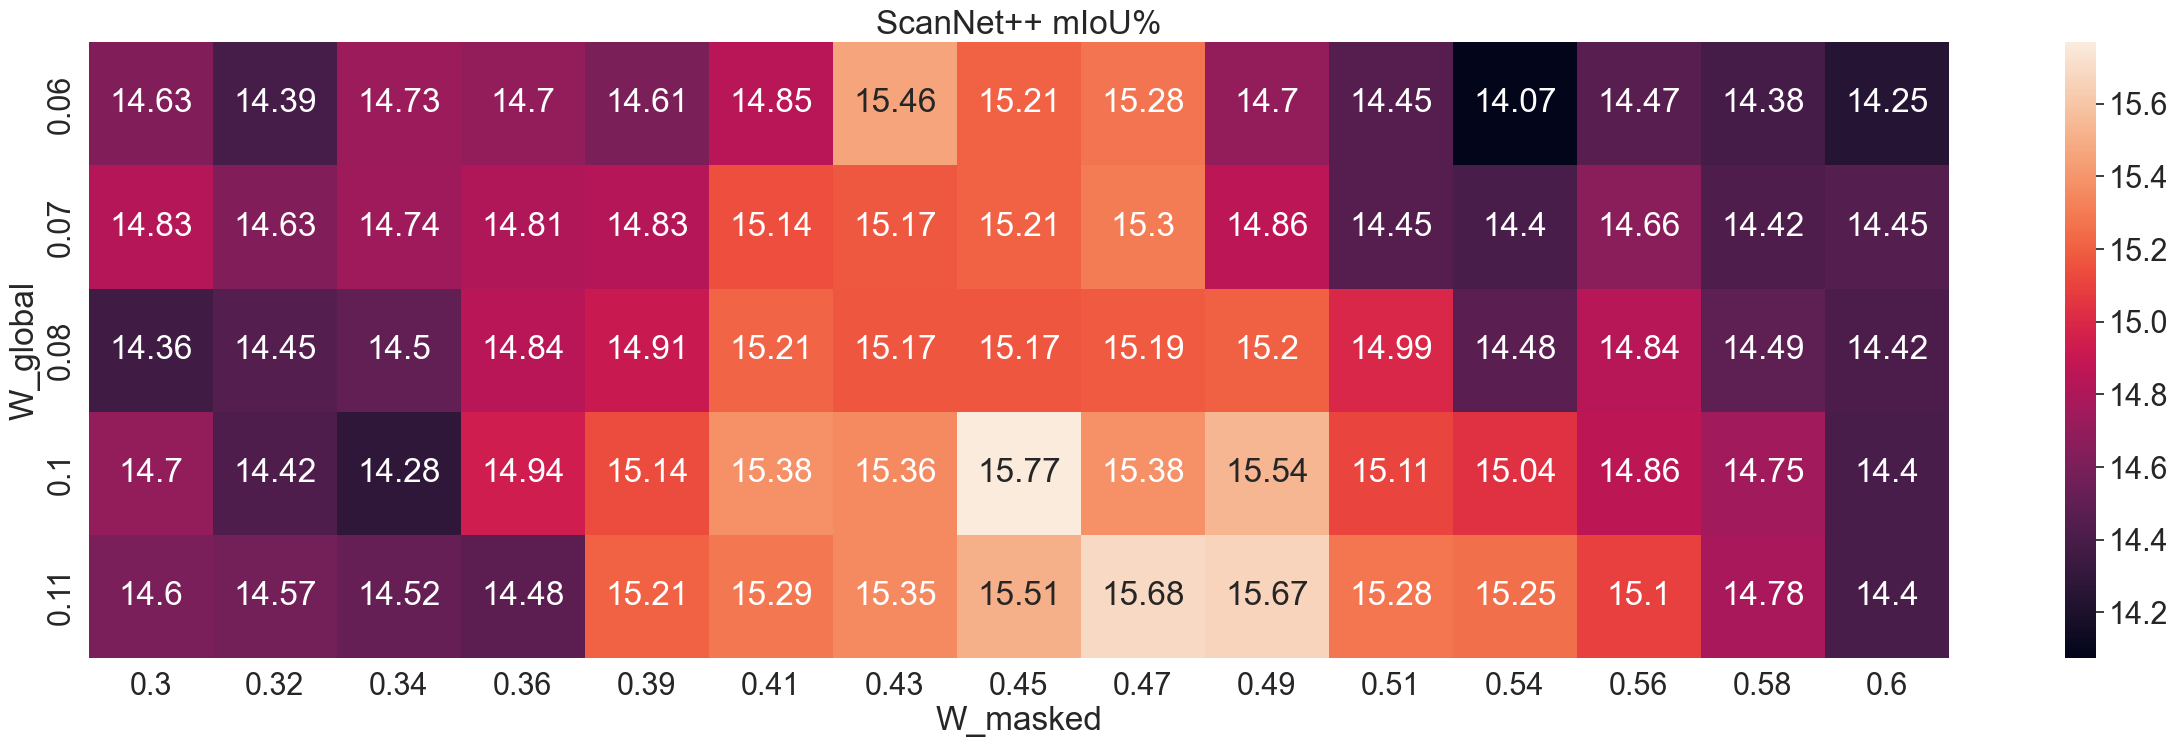
\includegraphics[width=\textwidth]{figures/ablation/clip_w_grid_search_scannetpp.png}
  \caption{{Grid search for CLIP weights merging on five scenes from ScanNet++~\cite{yeshwanthliu2023scannetpp}.}}
  \label{fig:w_grid_search}
\end{figure*}
\section{System ablations}
In this section we report minor ablations and experiments performed during \ours's development using ScanNet++ training set.
First we report an ablation of different foundation models for 2D instance segmentation, and language-image features extraction.
Then, we ablate the algorithm to merge different CLIP descriptors and validate our proposed \clipours.
We profit from the \clipours to reduce the number of CLIPs descriptors computations and evaluate the impact of the number of views on the selection of the final descriptor of 3D instances.
After that, we present a mask bleeding problem that arises from depth estimation inaccuracies, and how we tackled it.
Finally, we report an overall profiling of the system using different previously ablated components.
\newline
While the segmentation backbones where ablated on a single scene from ScanNet++, we used an extended set of five scenes for CLIP~\cite{radford2021clip} models and similarity computation, to ablate the set of fixed weights, the evaluation of the number of viewpoints, and the mask bleeding.
Then we used a different set of 10 scenes for the overall profiling to avoid overfitting on the previous set.
Regarding \clipours training was done using the 230 scenes from ScanNet++ training set, and validation against baselines was performed on ScanNet++ 50 scenes validation set, and on ADE20K-150.
We measured mean Intersection over Union (mIoU) of the 3D semantic segmentation.
\newline
As starting point, segmentation masks are computed using SAM 2~\cite{kirillov2023sam}; CLIP vectors are computed from masks using SigLIP-384; for each mask three vectors are computed and weighted together as introduced by HOV-SG~\cite{hovsg}; each 3D object gets assigned the CLIP vector from the view that minimizes the L1 distance to its other views. Finally semantic classes are matched to each 3D object using the similarity approach presented by LangSplat~\cite{qin2024langsplat}. 
%
\subsection{Foundation Models}
\paragraph{SAM} Since its release, Segment Anything Model (SAM)~\cite{kirillov2023sam} has been the state-of-the art for out-of-the box instance segmentation on different fields. Its segment-everything mode extracts multiple masks from a single image, taking an input a grid of point on the image. Nevertheless, this mode has a low throughput mainly due to the post-processing required to filter duplicated and bad segmentation masks.
Although several methods claim up to $\times 100$ speed-ups with respect to SAM, these speed-ups are measured when segmenting a single object on the image, and do not measure the segment-everything mode and its post-processing.
\newline
In this ablation the evaluated models are SAM~\cite{kirillov2023sam}, SAM 2~\cite{ravi2024sam2}, FastSAM~\cite{zhao2023fast}, and EfficientViTSAM~\cite{zhang2024efficientvit}.
The evaluation in ~\cref{tab:ablation_segment} shows how when segmenting everything these methods do not imply an improvement against a SAM implementation with tuned hyper-parameters. 
%\textit{From here on, all experiments will proceed using the recently released SAM 2}, which achieves the best balance between mIoU and latency. For the experiments in the main paper we use SAM 2.1, the latest checkpoint for SAM 2.
\begin{table}[h]
\centering
\small
\setlength\tabcolsep{9pt}
\caption{Segmentation backbone ablation.}
\begin{tabular}{lcc}
  \toprule
  & \multicolumn{2}{c}{281bc17764} \\ \cmidrule(lr){2-3} 
  SAM backbone & mIoU$\uparrow$ & Latency [s]$\downarrow$ \\ 
  \midrule
  FastSAM~\cite{zhao2023fast}    & 5.0 & \fs \(0.40\pm0.27\) \\ 
  EfficientViTSAM~\cite{zhang2024efficientvit} & 17.1 & \(4.19\pm0.85\) \\ 
  EfficientViTSAM~\cite{zhang2024efficientvit} - tuned & 15.1 & \nd \(0.68\pm0.05\) \\
  \midrule
  SAM~\cite{kirillov2023sam}         & \nd 19.0& \(5.43 \pm1.83\)  \\
  SAM~\cite{kirillov2023sam} - tuned & \rd 18.1 & \(0.84 \pm0.13\)  \\ 
  SAM 2~\cite{ravi2024sam2} - tuned & \fs 19.1 & \rd \(0.71\pm0.10\) \\ 
  \bottomrule
\end{tabular}
\label{tab:ablation_segment}
\end{table}
%
\begin{table}[ht]
\centering
\small
\setlength\tabcolsep{3pt}
%\resizebox{0.98\linewidth}{!}{
\caption{CLIP ablation results on 5 scenes from ScanNet++.}
\begin{tabular}{lccc}
\toprule
Architecture & Resolution& mIoU [\%] & Latency [s] \\
\midrule
DFN-ViT-B-16 & \multirow{5}{*}{\(224\times224\)} & 10.92 & \(\fs 0.100\pm0.022\) \\
DFN-ViT-L/14 &  & 11.89 & 
\nd \(0.173\pm0.031\) \\
DFN-ViT-H/14 &  & \rd 13.22 & \(0.286\pm0.054\) \\
OpenCLIP ViT-H/14 &  &  12.71& \(0.283\pm0.053\) \\
SigLIP-SO400M &  & \nd 13.78 & \rd \(0.229\pm0.026\) \\
\midrule
SigLIP-SO400M 384 & \multirow{2}{*}{\(384\times384\)} &  \fs 15.35 & \(0.442\pm0.080\) \\
DFN-ViT-H/14-378 &  &  12.96 & \(0.664\pm0.136\) \\
\bottomrule
\end{tabular}
%}
\label{tab:ablation_clip_arch}
\end{table}
%
\paragraph{Visual-Language descriptors.}
To compute image-language features we rely on the family of CLIP and its variants.
To select the CLIP architecture we evaluate the difference in performance and latency of different SOTA models to compute CLIP embeddings:
\begin{itemize}
  \item OpenCLIP~\cite{openclip_repo} base ViT-H-14, trained on LAION-2B English~\cite{schuhmann2022laion} at a resolution of \(224\times224\), using CLIP's cosine similarity.
  \item DFN~\cite{data-filtering-networks} ViT-B-16, ViT-L-14, and ViT-H-14 trained on the dataset DFN-5b~\cite{data-filtering-networks} with input images of \(224\times224\), and a ViT-H-14  finetuned at resolution \(384\times384\), using CLIP's cosine similarity.
  \item two SigLIP's Shape-Optimized 400M parameter ViT (ViT SO-400M), trained on WebLI English dataset at \(224\times224\), with one fine-tuned at \(384\times384\), and optimized using SigLIP's cosine similarity.
\end{itemize}
%
In this ablation each backbone is evaluated using the similarity with which they were trained, without ensembling, and using the template ``\textit{This is a photo of a \{class\}}''.
The results in ~\cref{tab:ablation_clip_arch} show a clear trade-off between segmentation performance, and model latency. SigLIP-384 achieves the best mIoU, while SigLIP at \(224\times224\) has the best balance between mIoU and speed.
Overall, this ablation shows the importance of selecting the proper CLIP backbone, with a difference of almost 5\% between the best and the worst model.
%
%
\subsection{CLIP descriptors merging}
\label{sec:supp_CLIP_merging}
\begin{figure*}[ht]
  \centering
    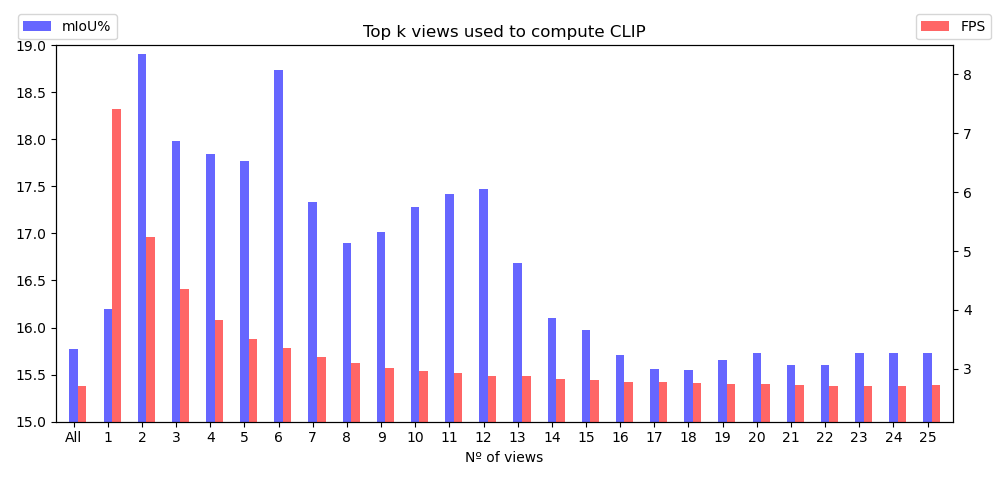
\includegraphics[width=0.9\textwidth]{figures/ablation/topk_miou.png}
  \caption{\textbf{Evaluation using only top views to compute CLIP on 5 scenes from ScanNet++~\cite{yeshwanthliu2023scannetpp}.} While using more than one view has substantial impact on the runtime, it also improves segmentation accuracy. However, too many views also degrade the segmentation accuracy. }
  \label{fig:topk}
\end{figure*}
%
\paragraph{Similarity computation.}
Initially, CLIP~\cite{radford2021clip} presented the cosine similarity, \(\cos\left(\phi_\text{qry},\phi_\text{img}\right)\) to compute the distance between the text, $\phi_\text{qry}$, and image, $\phi_\text{img}$, embeddings. SigLIP~\cite{zhai2023siglip} adapted it to its loss function, as \(\mathrm{Sigmoid}\left(\cos\left(\phi_\text{qry},\phi_\text{img}\right)\times \tau + b \right)\), including a Sigmoid operation, and the learned inverse temperature, \(t = \frac{1}{\tau}\), and bias \(b\) parameters. To classify, both approaches assigned to an image the class of the query that generated the highest similarity.
Also based on CLIP's experiments, to compute the cosine similarity HOV-SG~\cite{hovsg} computed query embeddings as \(\phi_\text{qry} = \frac{\phi_\text{cl}+\phi_\text{temp}}{2}\), where $\phi_{cl}$ is the text embedding computed from the class name, and $\phi_\text{temp}$ is the text embedding computed from the phrase resulting of inserting the class into the template ``\textit{There is \{class\} in the scene}''.
In contrast, LERF~\cite{lerf2023} proposed to compute the cosine similarity between the image and text embeddings as 
%
\begin{equation}
  \min_i \frac{\exp\big(\cos\left(\phi_\text{qry},\phi_\text{img}\right)\big)}{\exp\big(\cos\left(\phi_\text{qry},\phi_\text{img}\right)\big) + \exp\big(\cos\left(\phi_\text{can}^{i},\phi_\text{img}\right)\big)} \, ,
\end{equation}
%
where $\phi_\text{can}^{i}$ is the text embedding of one of the predefined canonical queries \textit{object, things, stuff, texture}.

\noindent
Using the SigLIP ViT-SO400M model to compute CLIP vectors, we compare between:
\begin{itemize}
  \item computing query embeddings, $\phi_\text{qry}$, only with the template  ``\textit{This is a photo of a \{class\}}'' or as an ensemble averaging the template embedding with the class embedding;
  \item and computing SigLIP's cosine similarity or LERF's cosine similarity.
\end{itemize}
Results in ~\cref{tab:ablation_sim} show how the basic configuration of using SigLIP similarity without ensemble achieves the best performance.
\textbf{From here on, all experiments will proceed using basic cosine similarity without ensemble.}
%
\begin{table}[]
\centering
  \caption{Similarity computation ablation on 5 scenes from ScanNet++ measuring semantic 3D mIoU.}
  \begin{tabular}{lcc}
    \toprule
                & Cosine similarity & LERF's similarity \\ \hline
  w ensemble    & 14.75\%           & 14.75\%         \\
  w\textbackslash o ensemble & \textbf{15.35\%}           & \bf 14.98\% \\ \hline       
  \end{tabular}
  \label{tab:ablation_sim}
\end{table}
\begin{table*}[]
%\vspace{-.6cm}
    \centering
    \small
    %\setlength{\tabcolsep}{1pt} % column spacing
%\resizebox{\columnwidth}{!}{%
    \caption{Our \clipours vs. baselines on: ScanNet++ (S++) using 1.6k queries (metrics on observed 495 labels, w. and w/o. the top 100 used at training), and ADE20k with 150 labels. Color indicates \colorbox{Green!25}{First}, \colorbox{SpringGreen!45}{second}, and \colorbox{Yellow!30}{third} best.}
\begin{tabular}{lccccccccccccc}
\toprule
 &\multicolumn{4}{c}{S++ w. top 100} &\multicolumn{4}{c}{S++ w/o. top100}&\multicolumn{4}{c}{ADE20k--150}\\ 
Method & mIoU & mAcc & f-mIoU &  \multicolumn{1}{c|}{f-mAcc} & mIoU & mAcc & f-mIoU &  \multicolumn{1}{c|}{f-mAcc} & mIoU& mAcc  & f-mIoU & f-mAcc\\
\midrule
HOV-SG & \nd 9.4 & \nd 15.9 & \rd 12.8 &  \multicolumn{1}{c|}{\rd 15.9}  & \fs 8.3 & \fs 15.1 & \nd 8.4 &  \multicolumn{1}{c|}{\rd 13.6} & \rd 21.9 & \nd 53.7& \rd 22.3  & \rd 34.9\\
%
Fixed-weights & \nd 9.4 & \nd 15.9 & \nd 13.1 &  \multicolumn{1}{c|}{\nd 16.3}  & \fs 8.3 & \fs 15.1 & \nd 8.4 &  \multicolumn{1}{c|}{\nd 13.8} & \nd 22.4 &\fs 53.9 & \nd 23.1 &\nd 35.5 \\
%
\bf CLIP-merger & \fs 10.7 & \fs16.9 &\fs 36.1 &  \multicolumn{1}{c|}{\fs 45.3} & \nd 7.3 & \nd 12.8 &\fs 9.9 &  \multicolumn{1}{c|}{\fs15.0} & \fs 23.4 & \rd 49.3 & \fs 28.7 & \fs 41.2 \\
\bottomrule
\end{tabular}%}
    \label{tab:clipmerger2}
    %\vspace{-0.6cm}
\end{table*}
%
%
\begin{table*}[]
\centering
\small
\setlength{\tabcolsep}{6.5pt} % column spacing
  \caption{\textbf{Average runtimes and 3D semantic performance on ScanNet++.} We measure the segmentation (Seg); segments matching and tracking (M\&T); segments pre processing (PP); CLIPs computation (CLIP); and total seconds per key frame (\(s/KF\)). 
  }
\begin{tabular}{clc|cccc|c|ccccc}
  \toprule
  CLIP & SAM & \# best views & Seg. [s] & M\&T [s] & PP [s] & CLIP [s] & \(s/KF\) & mIoU & mAcc & f-mIoU & f-mAcc \\
  \hline
  \multirow{2}{*}{ViT-H/14} & 1-H & \multirow{2}{*}{10}  & 1.516  & 0.269  & 0.085  & \nd 0.175  & 2.112  & 13.3 & 22.4 &20.2 & 31.7 \\\cline{2-2}
  &  2.1-L & & \rd 0.338  & \nd 0.252  & \rd 0.066  & \fs 0.135  & \nd 0.865  & \rd 14.1 & 24.9 &  27.3 & 37.7 \\\midrule
  \multirow{3}{*}{SigLIP} &  2.1-t &  \multirow{2}{*}{10} & \fs 0.245 & \fs 0.247  & \fs 0.057  & \rd 0.204  & \textbf{0.820}  & 11.8 & \rd 25.7 & \rd 34.2 & 
  \nd 46.6  \\ \cline{2-2}
  &  \multirow{2}{*}{2.1-L} & & 0.339  & \rd 0.253  & \nd 0.065  & 0.233  & \rd 0.957  & \nd 14.2 & \nd 27.0 & \nd 34.3 & \rd 45.6 \\\cline{3-3}
  &    & all & \nd 0.337  & 0.261  & 0.110  & 0.367  & 1.167  & \fs 15.8 & \fs 29.6 & \fs 36.3 & \fs 48.6 \\ 
  \hline
  \end{tabular}
  \label{tab:ablation_backbones}
\end{table*}
%
To focus CLIP descriptors to elements in an image, we follow HOV-SG's~\cite{hovsg} approach.
For each mask segmented by SAM, HOV-SG proposed to compute CLIP embeddings combining the information of the complete image, the masked image without background, and a bounding box of the mask including background.
For each segmentation mask $i$, its corresponding CLIP vector $F_i$ is computed as
%
\begin{equation}
F_{i} = F_\text{global} \times w_\text{global} + F_{\text{local}_i} \times (1 - w_\text{global}),
\end{equation}
with 
\begin{equation}
F_{\text{local}_i} = F_{\text{masked}_i} \times w_\text{masked} + F_{\text{bbox}_i} \times (1-w_\text{masked}),
\end{equation}
%
combinig the CLIP vector of the whole image, $F_\text{global}$, the CLIP vector of only the segmentation mask without background, $F_{\text{masked}_i}$, and the one of the bounding box of the segmentation mask including background, $F_{\text{bbox}_i}$.

HOV-SG~\cite{hovsg} used
\begin{equation}
  w_\text{global}= \mathrm{Softmax}(\cos(F_\text{global},F_{i})),
\end{equation}
%
and $w_\text{masked} = 0.4418$. 
Nevertheless, the use of the $\mathrm{Softmax}$ introduced a dependency between the different embeddings extracted on the same frame. To avoid computing all CLIP embeddings on every frame, we remove the $\mathrm{Softmax}$ and perform a grid search of \(w_\text{masked}\) and \(w_\text{global}\).
The best performance is achieved for \(w_\text{global} = 0.45 \text{ and } w_\text{masked} = 0.0975\) as shown in ~\cref{fig:w_grid_search}.
\paragraph{\clipours}
Rather than relying on 3 fixed-weights that ideally should be tunned for each scene, we developed the \clipours to estimate the corresponding weight for each image.
After training on ScanNet++ train set with the top 100 semantic labels, we evaluate its performance on the ScanNet++ validation set using the total set of 1.6k queries, both including (w.top 100) and excluding (w/o. top 100) classes seen during training. For a stronger distribution switch, we also evaluate on ADE20k-150.
\newline
Comparing its performance against HOV-SG's approach and our variation of HOV-SG's using three fixed weights, the \clipours outperforms the baselines using all the labels, \cref{tab:clipmerger2}. 
Excluding from the metrics the 100 labels seen during training, we can observe how the \clipours performance drops with respect to the baselines.
Despite the slight bias toward classes at training, it still outperform on freq. weighted metrics of classes that weren't seen during training, and on novel data on the ADE20k-150 dataset.
\newline
Although, \ours-mapping evaluation in Replica and ScanNetv2, additional segmentation metrics on classes outside the training set (\cref{tab:miou_macc} showcase how the bias does not have an impact on our \clipours's generalization.
Our method accurately detects in 3D several unseen classes across Replica and ScanNetv2, including \textit{guitar}, \textit{coffee maker}, \textit{blackboard}, and \textit{scale}. The mIoU for these examples exceeds 60\%. 
\textbf{From here on, all experiments will proceed using the \clipours.}
\begin{table}[t]
%\vspace{-4pt}
\centering
    \small
    \setlength{\tabcolsep}{3pt} % column spacing
    \caption{\textbf{\clipours generalization.} 3D metrics on ScanNetv2 of some classes not seen during training.}\label{tab:miou_macc}  
\begin{tabular}{lcccccc}
\toprule
 & \multirow{2}{*}{scale} & toaster  & \multirow{2}{*}{blackboard} & coffee  & \multirow{2}{*}{guitar} & projector  \\ 
 &  & oven &  & maker &  &  screen \\ \hline
mIoU\% & 75.1 & 78.53 & 61.4 & 67.0 & 62.68 & 64.1 \\% \hline
mAcc\% & 81.2 & 94.07 & 76.1 & 86.7 & 86.79 & 86.8 \\
\bottomrule
\end{tabular}
\end{table}
\subsection{Additional heuristics}
\paragraph{Nº of best views.}
%This ablation is also performed on a set of 5 scenes from ScanNet++ using SAM-2, SigLIP-384, and \ours mapping. 
To reduce the expensive CLIP computation for each frame, we evaluate the impact of using only the best views where each 3D segment has been seen to compute its CLIP descriptor.
We evaluate from using only the best image to using all the images where the object has been seen.
The quality of an image is based on the area of the object's 2D segmentation in it.
\newline
For a sequence of 51 keyframes, we evaluate for \(k\in\{1,\ldots,51\}\), being \textit{all} using all the views to compute objects 3D vectors. 
The results show, see ~\cref{fig:topk}, that neither using only the best nor using all the views are robust enough to noise. 
For the set of 5 scenes on this experiment, the best values of \(k\) are between 2 and 7, achieving an mIoU around 18\%, almost 3 points better than using all observations, although, the perfect value of will probably be scene and object dependent.
We decide to set use 10 views as a balance to avoid useless computation of CLIP vectors and being resistant to noisy images.
%
\paragraph{Masks bleeding.}
Observing OVO-SLAM matching results, we noticed some problems related with SAM's masks. When some 3D points are projected on the edges of a 2D mask to which they do not belong, they are wrongly clustered into it and matched to a 3D instance. Then, when these  are seen again they will propagate the wrongly assigned ID.
This phenomenon can be observed in particular on the edges of objects, where the depth and masks are less accurate, and masks propagate the ID of the object to the background, as seen in~\cref{fig:mask_bleeding}.
To compensate it we developed two approaches:
\begin{itemize}
  \item First, we add a filter to only keep matches of 3D points that are assigned to the same object in two consecutive frames;
  \item Second, we apply a low-pass filter to the depth map to mask the edges of the objects and avoid matching points around them.
\end{itemize}
Results on ~\cref{tab:ablation_depth_kf} show how while using the depth filter does improve the average mIoU, the limitation to match in consecutive frames does not. As a consequence we keep only the depth filter although it does not completely solve the problem.
%
\begin{table}[ht]
  \centering
  \setlength\tabcolsep{28pt}
  \caption{{Mask bleeding solutions' ablation on 5 scenes from ScanNet++~\cite{yeshwanthliu2023scannetpp}.}}
  \begin{tabular}{lc}
    \toprule
    Config & mIoU$\uparrow$ \\ 
    \midrule
    Base                    & \rd 15.80\% \\ 
    w depth filter          & \fs 16.16\% \\
    w consecutive KF filter & 15.07\% \\
    w both                  & \nd 15.82\%   \\
    \bottomrule
  \end{tabular}
  \label{tab:ablation_depth_kf}
\end{table}
%
\begin{figure}
    \centering
    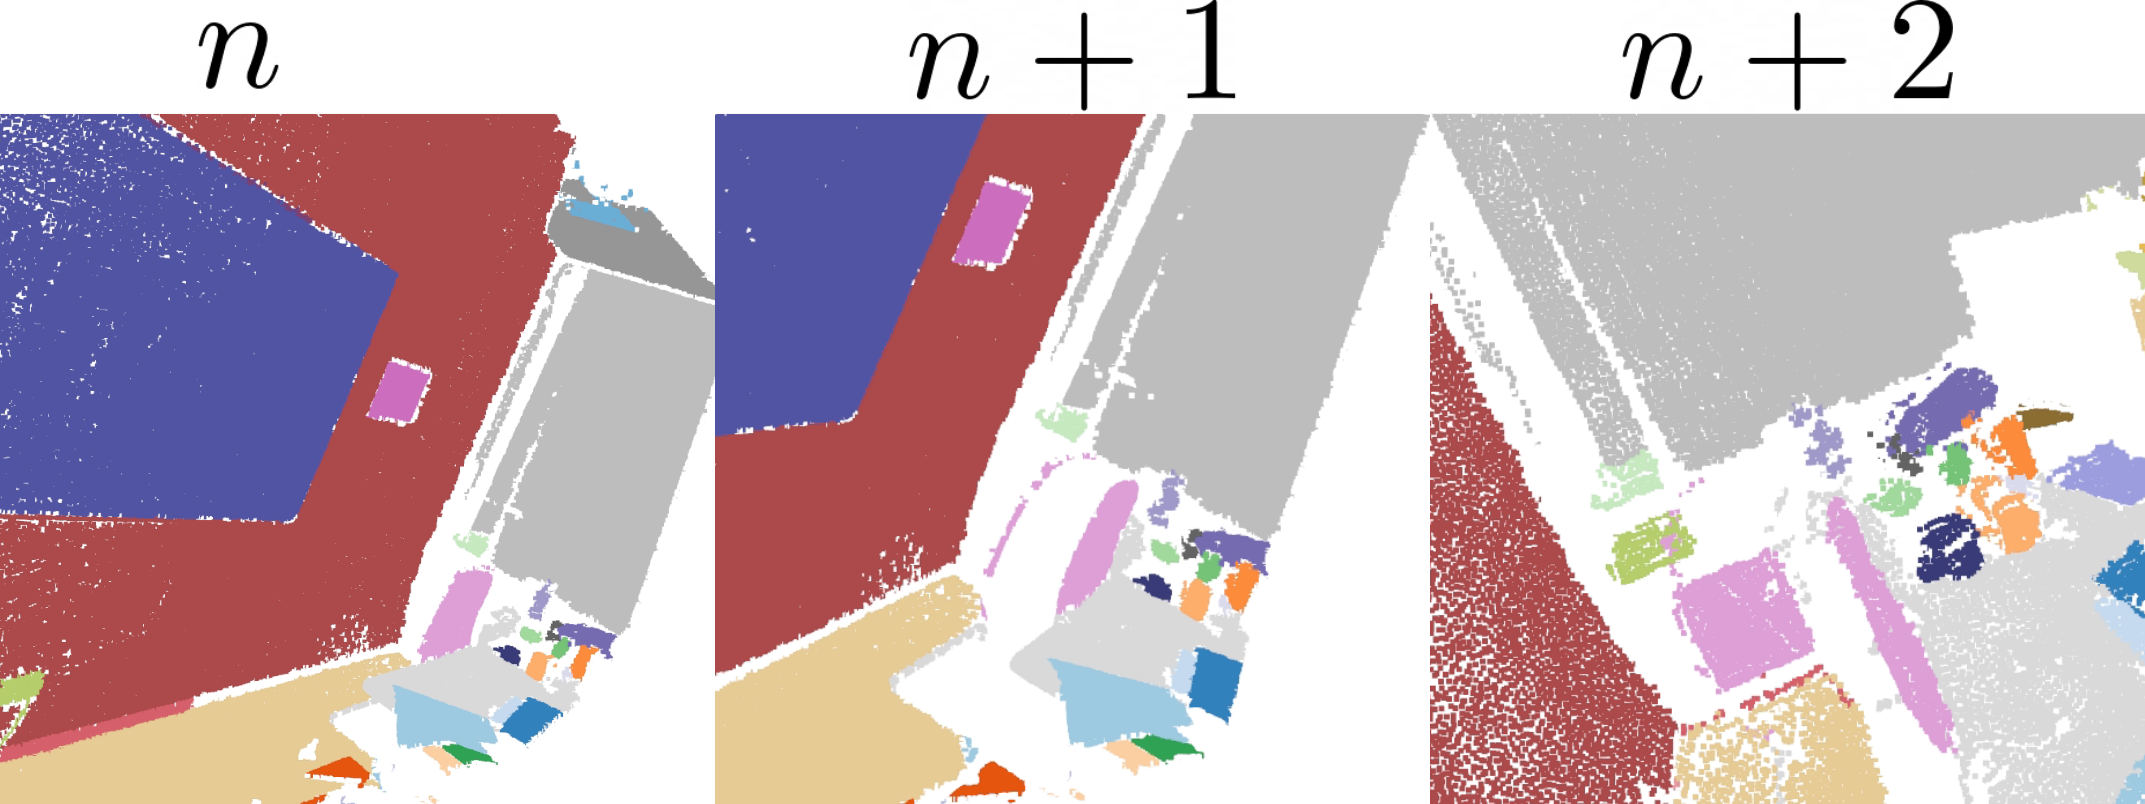
\includegraphics[width=\linewidth]{figures/images/mask_bleeding.png}
    \caption{\textbf{Mask bleeding} and propagation produced by masks inaccuracy. The edges of the chair (pink) bleed to the background at $k_n$, and therefore the segment label is wrongly propagated to the it in the following keyframes.}
    \label{fig:mask_bleeding}
\end{figure}
%
\paragraph{Overall profiling.} 
Finally, we quantify the latency-quality trade-off in our architecture evaluating selected foundation models and number of views against less powerful alternatives.
This evaluation is performed on a different set of 10 scenes from ScanNet++ to avoid over-fitting to the previous 5 scenes.
For 2D segmentation we evaluate SAM~\cite{kirillov2023sam} with ViT-H/14 encoder (1-H), and SAM 2.1~\cite{ravi2024sam2} with Hiera large (2.1-L) and Hiera tiny (2.1-t) image encoders. 
For CLIP extraction, we evaluate DFN ViT-H/14-378~\cite{data-filtering-networks} and SigLIP-SO400~\cite{zhai2023siglip} both with input images of 384 pixels.
The results in \cref{tab:ablation_backbones} show that in this set of scenes the best 3D segmentation is achieved with the largest models using all points of view.
Nevertheless, the best trade-off can be achieved reducing the number of views and the CLIP model.
\begin{comment}
\begin{table}[t]
%\vspace{-0.65cm} 
\centering
\small
\setlength{\tabcolsep}{3.4pt} % column spacing
\begin{tabular}{l|c|c|c|c}
\toprule
Dataset    & avg / max vRAM & checkpoint  & KFPS& \#KF  \\ \midrule
Replica    & 4.2 / 8.1 [GB]& 12$\pm$1 [MB] & 0.5$\pm$0.2& 200$\pm$0\\
ScanNet    & 4.4 / 7.7 [GB] & 15$\pm$5 [MB] & 0.8$\pm$0.3 & 172$\pm$98   \\
\bottomrule
\end{tabular}
    \caption{\textbf{\ours-mapping footprint.} GPU vRAM, checkpoint size, keyframes per second and number of keyframes.}\label{tab:runtime} 
\end{table}
\end{comment}
